\section{Design and Implementation of \os}
\label{s:design-hetero-net}



\begin{figure}[t]
  \centering
  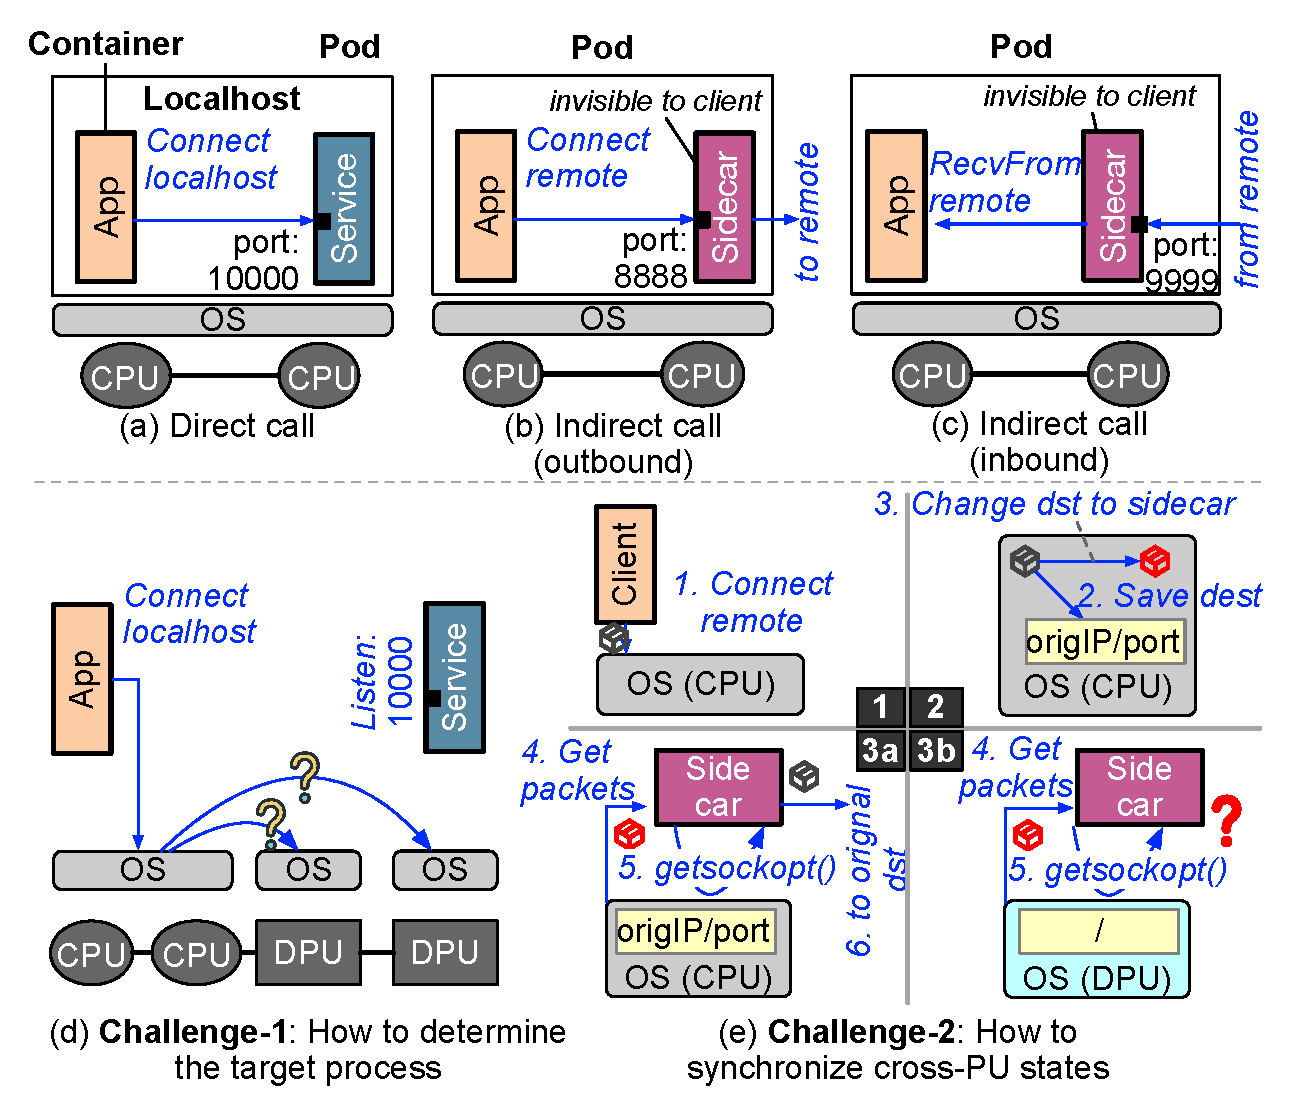
\includegraphics[width=0.48\textwidth]{figs/design-hetero-iptable.eps}
 \setlength{\belowcaptionskip}{-15pt}
 \setlength{\abovecaptionskip}{0pt}
  \caption{\textbf{Two types of network calls and challenges of split network namespace}.
  }
  \label{fig:hetero-splitns}
\end{figure}




\subsection{Split Network Namespace (\giptable)}
\label{subs:hetero-iptable}

\myparagraph{Notation.}
Network namespaces in Linux~\cite{net-ns} provide isolation of network-related system resources,
including network devices, protocol stacks, IP routing tables, port numbers and so on.
We extend the concept to \emph{split network namespace}, which provides a unified and isolated network abstraction
in a CPU-DPU computer.
Split network namespace can be exclusively used by one container (multiple processes) or can be shared by multiple containers (e.g., Kubernetes Pod).

\myparagraph{Network calls.}
We can classify network requirements into two types (Fig.\ref{fig:hetero-splitns}-a/b/c): \emph{direct call} and \emph{indirect call}.
Direct call indicates two processes within the network namespace can communicate by using \codeword{localhost} and port number.
Indirect call refers to the scenario where a message is not directly transmitted to a local receiver, 
instead, it is initially intended for a remote receiver but is then forwarded to a local receiver due to packet filtering rules, such as iptables or routing.

\myparagraph{Challenges.}
First, challenges arise when multiple kernels manage processes within the ``same'' network namespace.
For direct call, the sender's OS kernel faces the difficulty of \emph{determining which kernel} is responsible for the receiver's processes.
Naively, the OS kernel on the sender side could forward packets to the kernel on the receiver side, but the issue lies in the lack of information regarding which processes are deployed on which PUs, as shown in Fig.\ref{fig:hetero-splitns}-d.

Second,
indirect call further introduces a new challenge called \emph{state synchronization}, where OS kernels on different PUs may explicitly synchronize certain states to process the packets accurately.
For example (Fig.\ref{fig:hetero-splitns}-e),
a sidecar proxy container is deployed to intercept incoming and outgoing packets from application containers.
Typically, this is accomplished by adding iptables rules to the network namespace of the Pod, redirecting packets sent by the application to the port where the proxy accepts them.
These iptables rules modify the destination IP and port information to match that of the proxy.
The OS kernels store the original destination IP/port information for future reference (Fig.~\ref{fig:hetero-splitns}-e, step-2/3).
Upon receiving the packet, the proxy container applies filtering processes and utilizes the \codeword{getsockopt()} syscall to retrieve the original destination IP/port information (Fig.~\ref{fig:hetero-splitns}-e, step-4/5).
A naive solution would be to add a similar rule on the sender side (i.e., the application container) to modify the destination IP and port, changing them to match the desired receiver's PU.
However, this poses a challenge because the proxy container (located on another PU) cannot retrieve the original IP and port information.
The sender's OS kernel (CPU in the fig), rather than the receiver's (DPU in the fig), stores this crucial data.
Although it is possible to synchronize the data between two PUs, it is very hard in practice because of the complicated rules and states.

\subsubsection{Port-based Reverse Mapping}
We have observed that in a split network namespace, processes distributed across different PUs still \emph{share the same logical port space}.
Each port number can only be exclusively used by one process.
Building on this observation, we propose the design of \emph{port-based reverse mapping}.
This approach involves maintaining a reverse mapping table that keeps track of the port numbers and their corresponding PUs. The mapping is globally shared by all \os daemons on each PU.
When a container needs to use a port number, the \os daemon checks the table to ensure that the port number is available. If the port is already in use, the operation will fail.

To avoid the overhead of port synchronization and checking during the data plane, \os adopts a plane decoupling approach.
When there are changes in port information, the \os daemon generates and applies a set of single-PU packet filtering rules, primarily utilizing iptables and routing in the prototype.
These rules automatically detect the \emph{remote port number} and employ DNAT (destination NAT) and SNAT (source NAT) techniques to correctly forward the packet to the appropriate PUs.
As a result, both the sender and receiver processes remain unaware of these underlying changes and can continue communicating using \codeword{localhost} with (almost) zero cost as if nothing has changed.

\subsubsection{Partially Idempotent Packet Rules}
To overcome the second challenges, we propose \emph{partially idempotent packet rules}.
Specifically, instead of performing the packet rules only in the source PU and synchronize the states latter (which is hard),
we transfer the original rules into two sets of new rules that will be applied to source and destination PUs.
These rules may have \emph{redundant} operations to a packet, but not introduce new side effects (i.e., \emph{idempotent} in this case).
States can be synchronized automatically by re-doing operations in both PUs.

For example, in the case of Fig.\ref{fig:hetero-splitns}-e, instead of simply changing the dst to receiver's IP/port and saving the orig-dst in the sender's PU,
we split it into three rules (simplified):
(1, on sender's PU) routing the pkt from sender's PU to receiver's PU which will not change the pkt,
(2, on receiver's PU) routing the pkt to the receiver's container,
and (3, on receiver's PU) changing the dst and save the orig-dst.
These rules perform redundant operations --- (1/2) and (3) both moving the pkt to the receiver PU, however, it will not change the behavior but achieve states synchronized.
As indirect call is achieved through network rules, \giptable can detect and replace them with the new rules for interception about incoming and outgoing traffic.

\subsection{Elastic and Efficient XPU Networking}
\label{subs:hetero-socket}



\begin{figure}[t]
 \setlength{\belowcaptionskip}{-10pt}
 \setlength{\abovecaptionskip}{0pt}
  \centering
  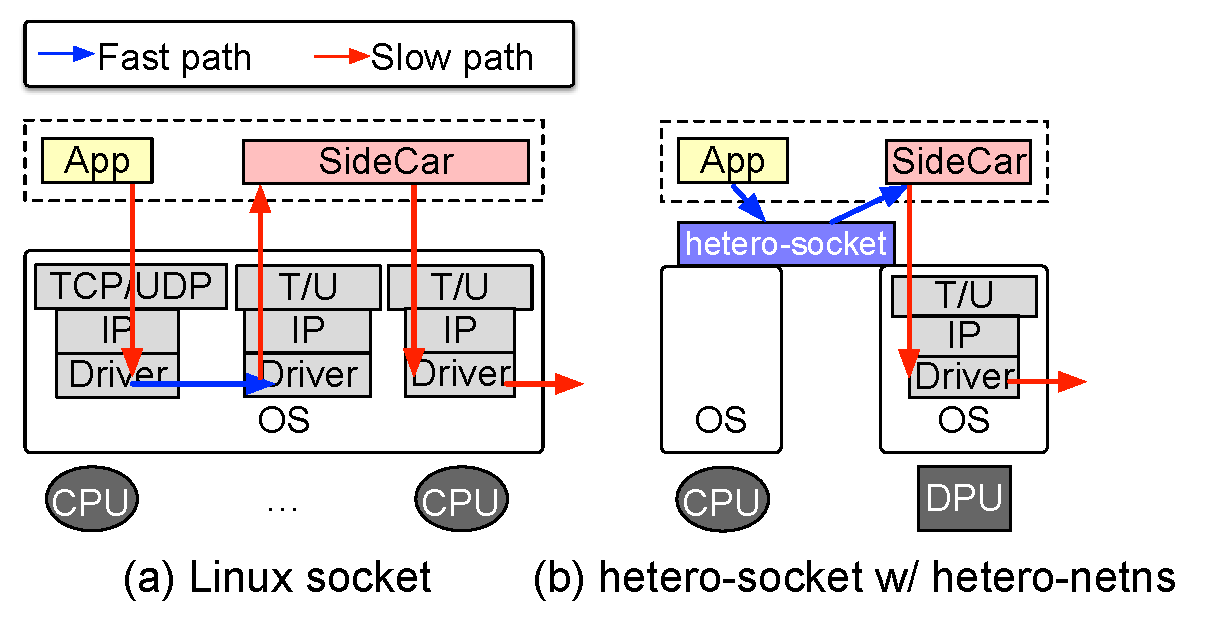
\includegraphics[width=0.45\textwidth]{figs/design-heterosocket.eps}
  \caption{\textbf{Communication path with infra-containers.}
}  
  \label{fig:design-heterosocket-netstack}
\end{figure}

\subsubsection{Overview}

Traditional network stack introduces unncessary redundancy for XPU communication which causes longer latency and restricts the optimization opportunities of fast interconnect.
For example, in microservice with sidecar, a message has to go through the network stack three times to arrive at its destination,
as shown in Fig.~\ref{fig:design-heterosocket-netstack}.
Although there are kernel-bypass socket-compatible systems~\cite{f-stack, dpdk, libvma}, they suffer poor resource utilization because of pinned memory buffer and static allocation (\textsection\ref{subsubs:hetero-socket-challenges}).
\gsocket aims to achieve the same performance as prior kernel-bypass design, but overcoming the resource challenges in the XPU setting.

\myparagraph{Cross-PU interconnects as global shared memory.}
We summarize one key primitive for XPU communication, \emph{global shared memory} (or GShm),
which means there would be a shared memory that can be used as a channel for cross-PU communication.
This assumption already holds for existing DPUs~\cite{mellanoxbf, marvel-liquidio}, e.g., Bluefield-2 supports RDMA to allow CPU and DPU to share an explictly allocated region.
To be general to different interconnects, \gsocket introduces an IAL (interconnect abstraction layer), which abstracts the interconnect details but only expose GShm abstractions to the core of \gsocket.

\myparagraph{Decoupling of control and data paths.}
\gsocket relies on Linux network stack to establish a connection (with \giptable),
and will form a GShm-based channel for the best performance when available.
During runtime, the data-path APIs like \emph{read()} and \emph{write()} will be intercept using GShm when possible, but apps can still utilize control path operations like \emph{getsockopt()} to get the metadata for a connection.
When containers are deployed on different PUs, \gsocket relies on sockets and \giptable to establish a correct connection and then utilizes the GShm to boost communication.



\subsubsection{Challenges}
\label{subsubs:hetero-socket-challenges}
Although kernel-bypassed and shared memory-based design is quite common can achieve best performance by fully utilizing hardware capabilities,
\sys aims to further resolve two technical challenges which are not resolved yet.
First (\textbf{Pinned resource costs}), the allocation of shared memory regions is usually privileged operations that require the OSes of two PUs to negotiate using interconnect primitives.
This procedure is usually slow (e.g., RDMA~\cite{280746}), making dynamically extend the regions hard.
As a result, existing systems tend to \emph{reserve} a fixed size of region in OS for a connection to use, facing the trade-off between resource wastes and performance slowdown.
The issue is significant in real-world as there may be thousands of connections in a machine. 
Second (\textbf{Polling costs}), as OS kernel is bypassed, user-mode stacks are responsible to explictly poll the data, leading to an old trade-off between PU costs and long latency.


\subsubsection{User-mode Resource Management with Speculative Allocation}
\label{ss:spec-alloc}

\gsocket employs an OS-library co-design for efficient memory management (Fig.~\ref{fig:design-heterosocket-umem}).
The core abstraction is the \emph{record} --- a page-aligned buffer with metadata (e.g., \emph{nextRecord}), unidirectionally accessible by either sender or receiver processes.
Each connection maintains two local records (one per direction) and leverages per-core \emph{shared arenas} containing dynamically allocatable records, managed as a list with \emph{headRecord} and \emph{tailRecord}.
This hybrid approach balances performance (local records) and scalability (shared arenas) while addressing three key challenges:

\myparagraph{Isolation \& synchronization.}
Shared arenas require strict access control: processes may only access their connection's records or their core's free records. \gsocket enforces this via memory mapping – during scheduling, the OS maps (1) local records, (2) occupied shared records for active connections, and (3) core-local free records. Per-core arenas eliminate synchronization overhead as free records are exclusively accessible during a process's time slice.

\begin{figure}[t]
  \setlength{\belowcaptionskip}{-10pt}
  \setlength{\abovecaptionskip}{5pt}
  \centering
  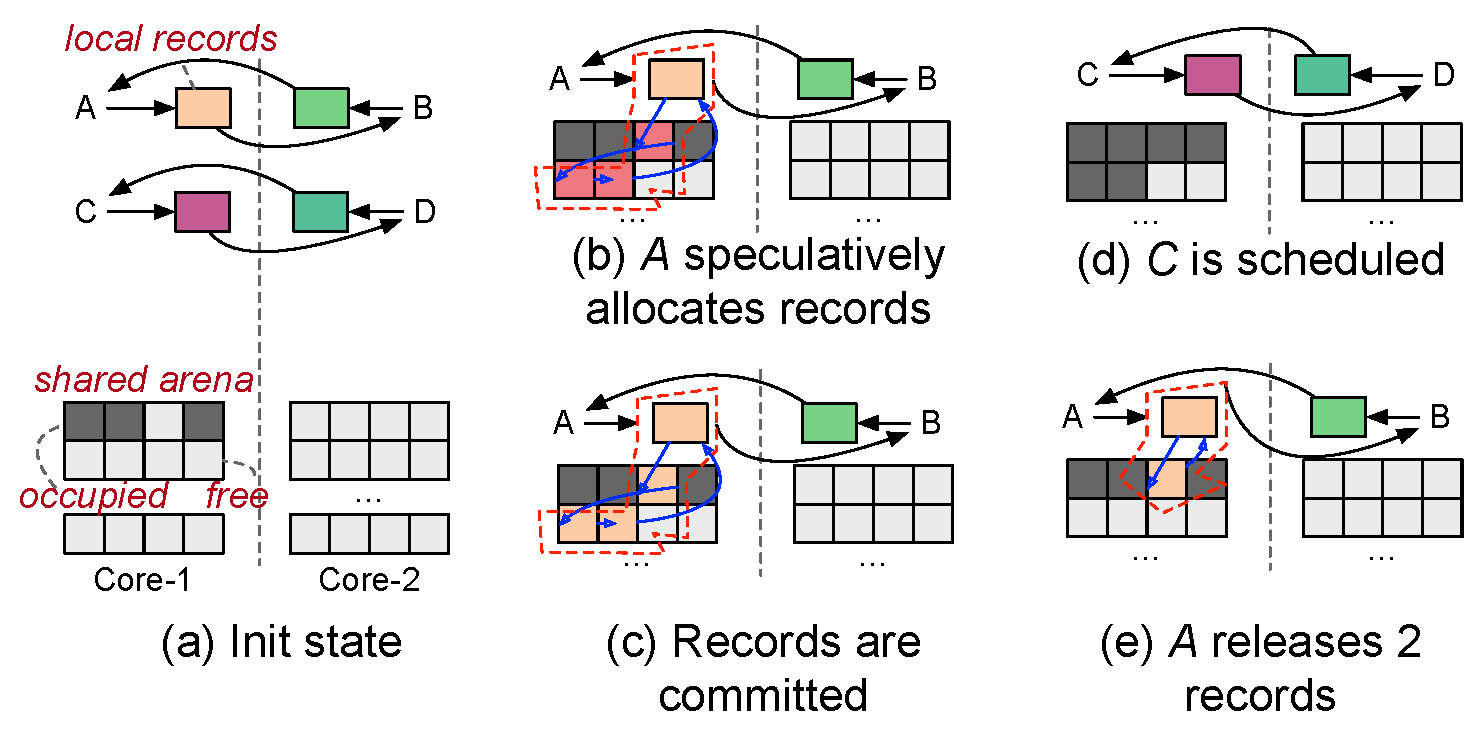
\includegraphics[width=0.47\textwidth]{figs/design-umem.eps}
  \caption{\textbf{Speculative allocation workflow} (a) record and arena, (b) speculative allocation, (c) kernel commit, (d) access control, (e) release.}
  \label{fig:design-heterosocket-umem}
\end{figure}

\myparagraph{Dynamic record chaining.}
Records form linked lists via a \emph{nextRecord} metadata. When a sender exhausts buffer space, it speculatively appends free records from its core's arena without kernel involvement (Fig.~\ref{fig:design-heterosocket-umem}-b).
The kernel later commits these allocations during context switches or exceptions (e.g., page faults) by remapping records as occupied (Fig.~\ref{fig:design-heterosocket-umem}c-d).
This two-phase approach --- user-space speculation followed by kernel ratification –-- achieves kernel-bypass performance with 64$\times$ less pinned memory (\S\ref{subs:eval-socket-microbench}).
For the receiver process of a connection, it may access a record that is newly allocated by the sender, which will trigger a page fault because of lacking permissions to access the free records.
In this case, the OS kernel will handle the page fault by mapping all newly allocated records to the receiver (also finishing the \textbf{commit}).
This trapping is rare in practice.


\myparagraph{Resource governance.} 
Rate-limiting policies prevent resource hoarding by bounding record usage per process.
The kernel enforces these during commit phases while preserving core-local allocation advantages.

\myparagraph{Design summary.} 
As a result, \gsocket can achieve similar resource management effectiveness as kernel-centric design except changing the gloabl resource pool to per-core pools (shared arena).
This change makes sense to avoid cross-core interferences and synchronization.
Compared with kernel-bypass network design with pre-reserved memory, \gsocket achieves similar performance as the trapping on the receiver side is very rare.
In fact, we even observe performance improvement as the dynamic resource of \gsocket can better dispatch resources among connections and better suit for varying loads.




\subsubsection{User-mode NAPI}
\label{ss:unapi}

\gsocket introduces the U-NAPI, a user-space adaptation of Linux's NAPI~\cite{linux-napi} that eliminates polling overhead through interrupt-driven event handling.
Traditional kernel-bypass designs waste CPU cycles polling for events --- U-NAPI instead dynamically switches between interrupt and polling modes based on traffic patterns, mirroring NAPI's adaptive behavior in OS kernels.

\myparagraph{Event management.}  
\gsocket keeps standard \codeword{epoll} semantics and adds two key syscalls: \codeword{enable\_notify\_gshm} and \codeword{disable\_notify\_gshm}. 
These allow applications to register interest in events (e.g., buffer availability) with the kernel.
\codeword{enable\_notify\_gshm} supports two modes (using different flags): \codeword{sync} and \codeword{async}.
The \codeword{sync} flag blocks threads until events occur (ideal for blocking I/O), while \codeword{async} triggers signal handlers that disable interrupts and enable polling for latency-sensitive phases.
The key innovation here is that U-NAPI leverages OS kernel to simulate the hardware to provide interrupt capability for U-mode event management.

\myparagraph{Integration with network operations.}  
In practice, U-NAPI optimizes three common scenarios.
First, a network \codeword{write} (or \codeword{send}) operation may block and turns to polling because the buffer of a connection is full.
In this case, the \gsocket uses \codeword{enable\_notify\_gshm(token, sync | W\_flag)},
which blocks in the kernel until the connection is ready for write.
Second, a similar case is blocking \codeword{read} (or \codeword{recv}) on an empty connection.
The \gsocket can use \codeword{sync} mode with \codeword{R\_flag}.
Last, to handle the case to add a new event to an epoll instance,
\gsocket can use \codeword{async} mode to monitor events, i.e., \codeword{enable\_notify\_gshm(token, async | events)}.
Then it can use the signal handler to handle any event updates, disabling notification, and turn to polling for performance.

\myparagraph{Cross-PU event propagation.}  
U-NAPI uses two cross-PU event delivery techniques.
First, \emph{proactive notification} has the remote side of a connection proactively tell the remote (or same PU) kernel of a new event. 
E.g., in blocking write, when the remote receiver reads data, checks status, and finds the sender blocked, it uses a syscall to tell the kernel the connection status changed, which eventually alerts the sender space may be available.
Second, \emph{Notify-on-RW (NoRW)} makes the kernel tell the remote (or same) kernel to revoke connection record permissions (e.g., no read-permission in the write case). This causes page faults on the receiver's read, which are sent to the sender's kernel to notify of the connection status change. 
Though cross-PU latency exceeds local cases, apps retain the flexibility to revert to polling for critical paths.



